\section{Segment}
\label{sec:Segment}

\begin{figure}[!ht]
\begin{center}
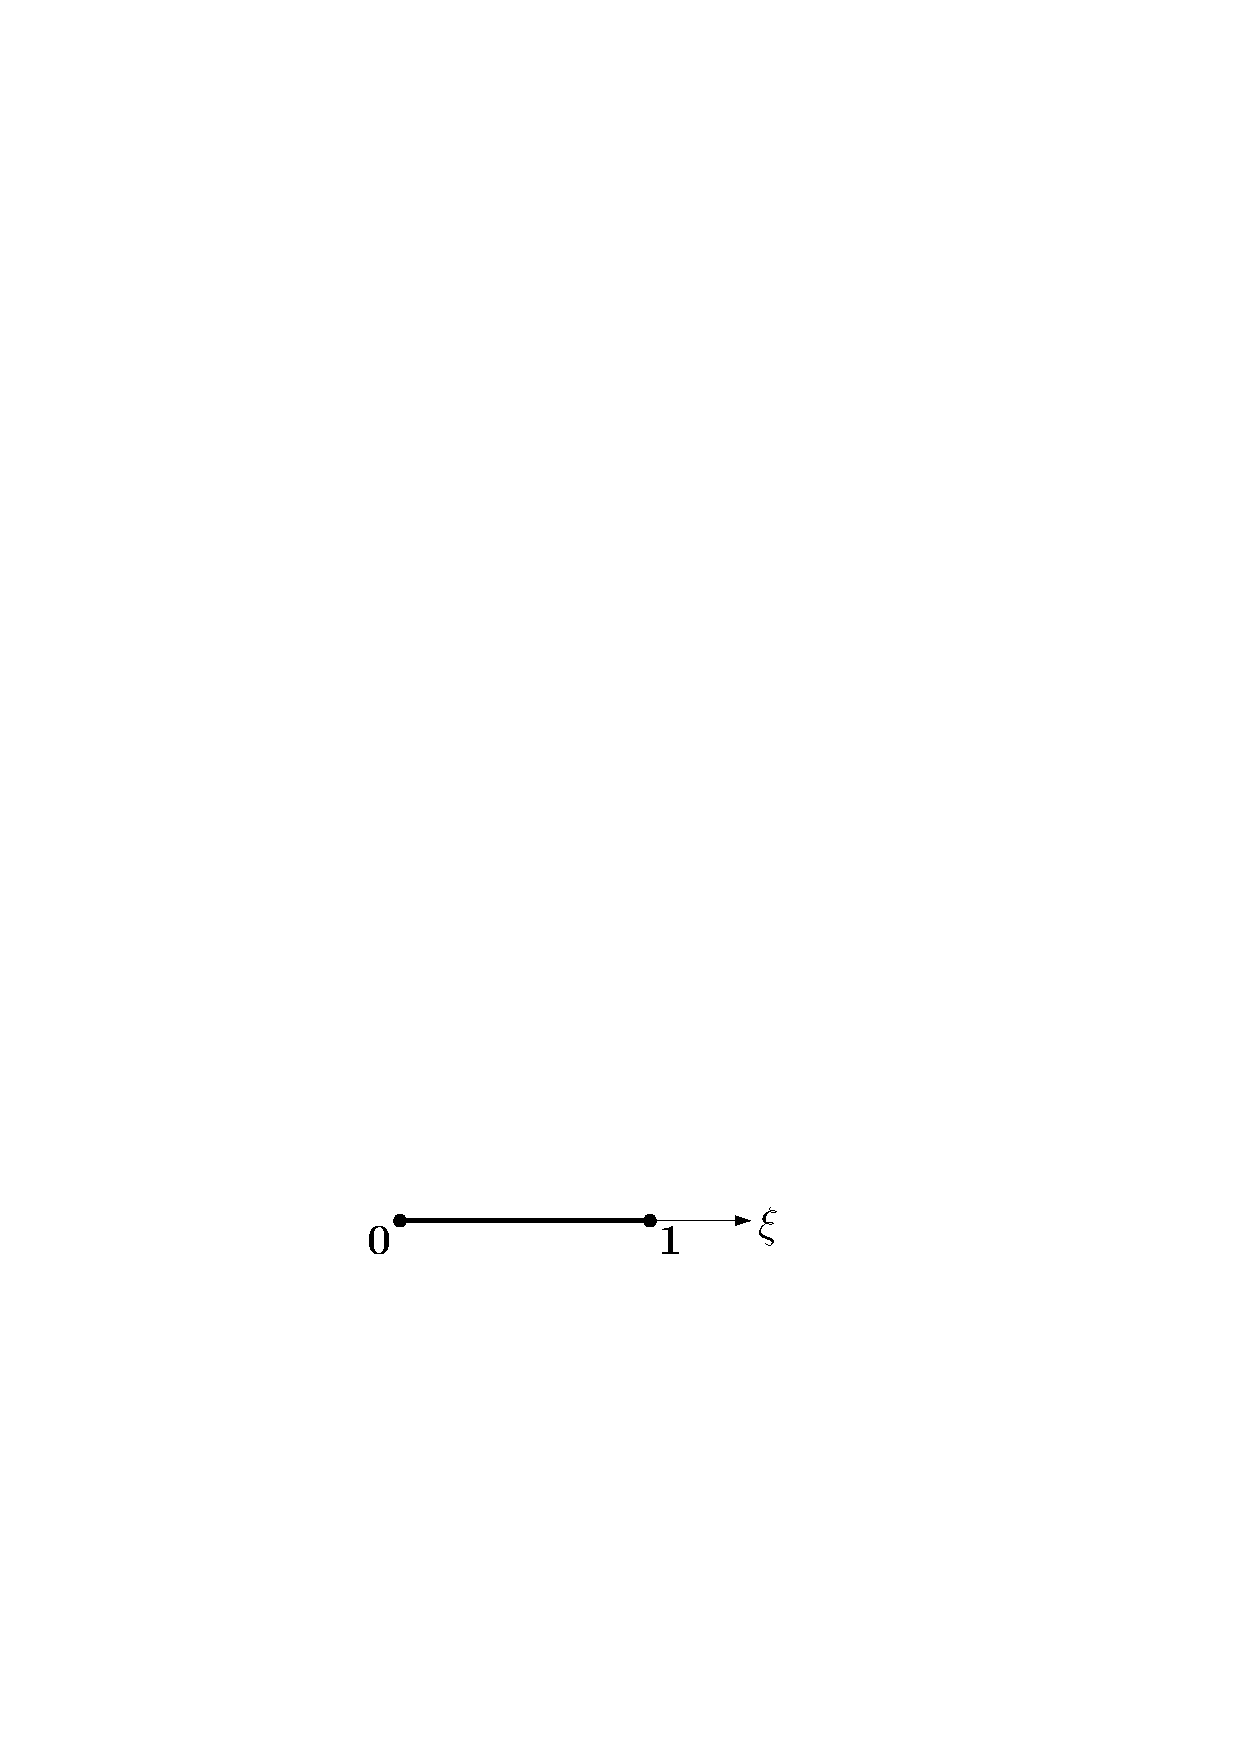
\includegraphics[scale=0.5]{./figures/MasterSegment.pdf}
\caption{Master segment with numbered vertices.}
\label{fig:masterseg}
\end{center}
\end{figure}

The 1D simplex is the segment or edge. 
The master element is defined as the unit interval $(0,1)$, and it is illustrated in Figure \ref{fig:masterseg} with a parameterization given by $\xi\in[0,1]$.

Denote vertex $a$ by $v_a$.
The definition of affine coordinates (see \eqref{eq:affinerepresentation}) states that $\xi=\mu_0(\xi)v_0+\mu_1(\xi)v_1$, with $\mu_0(\xi)+\mu_1(\xi)=1$, $\mu_0(\xi)\geq0$ and $\mu_1(\xi)\geq0$ for all $\xi\in[0,1]$.
Hence, $\mu_0$ is the weight related to $v_0$ and $\mu_1$ is the weight related to $v_1$.
For our master element, $v_0=0$ and $v_1=1$.
It then follows that the 1D affine coordinates for the segment, $\mu_0,\mu_1$, are the most basic linear functions.
They are written explicitly below for our master element:
\begin{equation}
		\mu_0(\xi) = 1 - \xi\,,\qquad\qquad \mu_1(\xi) = \xi \,.\label{eq:H1_1DAffine}
\end{equation}
%As expected, $\mu_0(\xi)+\mu_1(\xi)=1$, where $\mu_0(\xi)\geq0$ and $\mu_1(\xi)\geq0$ for all $\xi\in[0,1]$. 
The gradients of the affine coordinates (in 1D) are
\begin{equation}
		\nabla\mu_0(\xi)=-1\,,\qquad\qquad\nabla\mu_1(\xi)=1\,.\label{eq:gradH1_1DAffine}
\end{equation}
%Denote vertex $i$ by $v_i$, and recall that in the definition of affine coordinates (see \eqref{eq:affinerepresentation}), $v_0$ is coupled with $\mu_0$, while $v_1$ is coupled with $\mu_1$. 


\subsubsection*{Exact Sequence}
%The exact sequence for $\e$ is, by far, the most simple of all of the elements. It is well known that $L^2$ functions are realized as gradients of $H^1$ functions, and so the one dimesional sequence
%\begin{equation}
%% \mathbb{R} \xrightarrow{\text{Id}}
%H^1 \xrightarrow{\nabla} L^2
% % \xrightarrow{0} \{0\}\,,
%\label{eq:1DExactSeq}
%\end{equation}
%is exact. Here, the gradient is simply differentiation in a single variable.
The 1D exact sequence can be consulted in \S\ref{sec:Exactsequences}. 
Polynomial spaces are subsets of both $H^1$ and $L^2$ (in $(0,1)$), so we may consider a truncated polynomial approximation (of order $p$) to $H^1$ and induce a new (discrete) polynomial exact sequence
\begin{equation}
	\mathcal{P}^p \xrightarrow{\nabla} \mathcal{P}^{p-1}\,,\label{eq:ESsegment}
\end{equation}
where $\mathcal{P}^p=\mathcal{P}^p(\xi)$.
In the notation of \eqref{eq:polynomial_exact_sequences}, $W^p=\mathcal{P}^p$ and $Y^p=\mathcal{P}^{p-1}$.
%It is for each space in this sequence which we seek to create a basis of shape functions.

\subsection{\texorpdfstring{$H^1$}{H1} Shape Functions}

%In $H^1$ the trace is understood as the value of the function itself at the boundary. In the context of 1D, the boundary is simply the endpoints $\xi=0$ and $\xi=1$.
%In general, the {\em bubbles} are those functions with zero trace, so that in $\e$, the bubbles are those which vanish at the endpoints. Also, vertex functions should vanish at all other vertices.
The set of all shape functions defined in this section will form a basis for the space $\mathcal{P}^p$ which has dimension $p+1$.
In fact, there will be $2$ vertex shape functions and $p-1$ edge shape functions.
They will all be linearly independent and be contained in $\mathcal{P}^p$, so they will clearly form the desired basis.
% \paragraph{\texorpdfstring{$H^1$}{H1} Vertex Shape Functions and Bubbles.}

\subsubsection{\texorpdfstring{$H^1$}{H1} Vertices}

%We denote by $\mu_0,\mu_1$ the standard linear shape functions,
%They are actually 1D affine coordinates, since $\mu_0(\xi)+\mu_1(\xi)=1$, where $\mu_0(\xi)\geq0$ and $\mu_1(\xi)\geq0$ for all $\xi\in\e$.
%For more details about affine coordinates see \textit{cite section triangles}.
%Their gradients in 1D are trivial:
%\begin{equation}
%    \nabla\mu_0(\xi)=-1\qquad\qquad\nabla\mu_1(\xi)=1.
%\end{equation}
As previously mentioned, each vertex is linked to an affine coordinate.
For instance, $v_0$ is linked to $\mu_0$.
It is then quite natural to consider the affine coordinate itself as the \textit{associated} vertex shape function to $v_0$:
\begin{equation*}
	\phi^\mathrm{v}(\xi)=\mu_0(\xi)\,.
\end{equation*}
Indeed, it satisfies all the desired trace properties, since it takes the value $1$ at $v_0=0$, and $0$ at $v_1=1$.
Moreover, it decays linearly to the other vertex, so that it lies in $\mathcal{P}^1$, and respects the hierarchy.
Having the vertex function of the form $\mu_0(\xi)^p$ instead, would give a (faster) nonlinear decay, but then the function would be dependent on $p$ and the hierarchy would be broken.

In general, the vertex functions, along with their gradients are,
%They are, along with their gradients,
\begin{equation}
    \phi^\mathrm{v}(\xi) = \mu_a(\xi)\,,\qquad \quad \nabla\phi^\mathrm{v}(\xi)=\nabla\mu_a(\xi)\,,
\end{equation}
for $a=0,1$. Clearly, there are a total of $2$ vertex functions (one associated to each vertex).

%Here, the vertex function $\phi^\mathrm{v}(\xi)=\mu_a(\xi)$ is \textit{associated} to vertex $a$, and as required, it takes the value $1$ at the associated vertex, $v_a$, and $0$ at the other vertex.
%Notice, they decay linearly towards the other vertex to respect the hierarchy, and indeed, they lie in $\mathcal{P}^1$.
%We could choose the vertex functions to be of the form $\mu_a(\xi)^p$, which gives a (faster) nonlinear decay, but then the vertex functions would be dependent on $p$, and the hierarchy would be broken.

\subsubsection{\texorpdfstring{$H^1$}{H1} Edge Bubbles}
Recall from \S\ref{sec:LegendrePol} that the Legendre polynomials are seen as elements of $L^2$ which have the zero average property (over $[0,1]$), so that the integrated Legendre polynomials (of order $2$ and higher) are elements of $H^1$ which vanish at $0$ and $1$ (see \eqref{eq:Lvanishatendpoints}).
These are precisely the desired characteristics for $H^1$ edge bubbles.
Hence, the edge functions are defined as:
\begin{equation*}
    \phi^\mathrm{e}_i(\xi) = L_{i}(\xi),\quad i=2,\ldots,p\,.
\end{equation*}
This formula is perfectly valid and quite simple.
However, along this document, the use of affine coordinates will be enforced as much as possible.
The reasons for this will become clear as we move into higher dimensions.
Indeed, notice that due to $\mu_1(\xi)=\xi$, one can write $L_i(\xi)=L_i(\mu_1(\xi))$.
Moreover, since $\mu_0+\mu_1=1$, by \eqref{eq:homogfor1Daffine} it follows
\begin{equation*}
	L_i(\mu_1)=L_i(\mu_1;1)=[L_i](\mu_0,\mu_1)\,.
\end{equation*}
With this in mind, consider the following more general setting.

\begin{definition*}
Let $s_0$ and $s_1$ be arbitrary functions of some spatial variable in $\R^N$, with $N=1,2,3$. Denote by $p_s$ the order in the coordinate pair $(s_0,s_1)$. Then
\begin{equation}
    \phi^\E_i(s_0,s_1) = [L_i] (s_0,s_1) = L_i(s_1;s_0+s_1)\,,
\end{equation}
for $i=2,\ldots,p_s$. The gradients, understood in $\R^N$, are
\begin{equation}
    \begin{aligned}
    \nabla\phi^\E_i(s_0,s_1)&=[P_{i-1}](s_0,s_1)\nabla s_1 + [R_{i-1}](s_0,s_1)\nabla (s_1+s_0)\\
        &=P_{i-1}(s_1;s_0+s_1)\nabla s_1 + R_{i-1}(s_1;s_0+s_1)\nabla (s_1+s_0)\,.
    \end{aligned}
\end{equation}
\end{definition*}

Clearly, the definition of $\phi_i^\E$, involving homogenization, can be thought of as an extension of our more simple case.
This is the first of the so-called \textit{ancillary functions} which are defined in this work.
It is highlighted as an important definition, because it will be used multiple times throughout the text in more general settings.
Here, the superscript $\E$ stands for \textit{edge}, and one should think of this topological entity when looking at this function.
Also, note its arguments, $s_0,s_1$, are meant to be affine coordinates (or at least affine-related).

Rewriting \eqref{eq:Lhomogvanishatendpoints}, it follows that for any $s_0,s_1$, and all $i\geq2$,
\begin{equation}
	\phi^\E_i(0,s_1)=\phi^\E_i(s_0,0)=0\,.\label{eq:phiEvanishing}
\end{equation}

As observed, when the coordinates are 1D affine coordinates, like in this case, the formulas for $\phi^\E_i$ and its gradient are simplified.
For this, record the next remark.

\begin{remark}
Let $\mu_0=1-\mu_1$, where $\mu_1$ is an arbitrary function of some spatial variable in $\R^N$, $N=1,2,3$, and where $p$ is the order in the coordinates $(\mu_0,\mu_1)$. Then for all $i=2,\ldots,p$,
\begin{equation}
    \phi_i^\E(\mu_0,\mu_1)=L_i(\mu_1)\,,\quad\qquad \nabla\phi_i^\E(\mu_0,\mu_1)=P_{i-1}(\mu_1)\nabla\mu_1\,.
    \label{eq:H11Dspecialcase}
\end{equation}
\end{remark}

From now on, shape functions will be written in terms of ancillary functions and the affine coordinates of the element being analyzed.
Indeed, all that is required to compute $\phi_i^\E$ and $\nabla\phi^\E_i$ are $s_0,s_1$ and $\nabla s_0,\nabla s_1$ (since we already know from \S\ref{sec:LegendrePol} how to compute the scaled versions of $L_i$, $P_i$ and $R_i$).
For the segment, $s_0=\mu_0,s_1=\mu_1$, so this information is in \eqref{eq:H1_1DAffine} and \eqref{eq:gradH1_1DAffine}.

At first, this approach might seem to be overcomplicated given the simplicity of the initial formula (which does not involve scaling).
However, computationally speaking, this motivates coding $\phi^\E_i$ and $\nabla\phi^\E_i$, which will be observed to be fundamental as the document progresses.
If desired, within the $\phi^\E_i$ subroutine, one could decide to separately handle the special situation where $s_0,s_1$ are 1D affine coordinates, in which case the simplification shown in \eqref{eq:H11Dspecialcase} would then hold.
More importantly, when orientations become relevant, they will be handled through permutations of the arguments of $\phi_i^\E$.
Hence, having everything written in terms of $\phi_i^\E$, and in general, in terms of ancillary functions, is highly desirable.

Recalling that $\vec{\mu}_{01}=(\mu_0,\mu_1)$, the shape functions and their gradients are then defined as
\begin{equation}
    \phi^\mathrm{e}_i(\xi) = \phi^\E_i(\vec{\mu}_{01}(\xi))\,,\qquad\quad
    	\nabla\phi^\mathrm{e}_i(\xi) = \nabla\phi^\E_i(\vec{\mu}_{01}(\xi))\,,\label{eq:phiEgeneral}
\end{equation}
for $i=2,\ldots,p$. There are $p-1$ edge bubbles for the segment.% These are \textit{the} 1D $H^1$ edge bubbles.

%Notice that this collapses to the original Lobatto polynomials written at the beginning:
%\begin{equation*}
%    \phi^\E_i(\mu_0(\xi),\mu_1(\xi))=[L_i] (\mu_0(\xi),\mu_1(\xi))=L_i(\xi;1)=L_i(\xi)\,.
%\end{equation*}
%The gradients are obviously the Legendre polynomials, and this is also reflected by the general formula:
%\begin{equation*}
%    \nabla\phi^\E_i(\mu_0(\xi),\mu_1(\xi))=P_{i-1}(\xi;1)\nabla\mu_1(\xi)+R_{i-1}(\xi;1)\nabla 1=P_{i-1}(\xi)\,.
%\end{equation*}
%Due to $i\geq2$ it is clear that $\phi^\mathrm{e}_i(0)=\phi^\mathrm{e}_i(1)=0$ by the properties of the Lobatto polynomials, so that they are indeed bubbles satisfying the vanishing trace properties.
As previously mentioned, it is clear that $\phi^\mathrm{e}_i(0)=\phi^\mathrm{e}_i(1)=0$, by the properties of the integrated Legendre polynomials when $i\geq2$ (see \eqref{eq:Lhomogvanishatendpoints} or \eqref{eq:phiEvanishing}).
Hence the trace properties are satisfied.

%However, it generalizes naturally as the number of spatial dimensions increase.
%In those cases the scaling will not be trivial.
%Also, computationally speaking, this approach motivates coding $\phi^\E_i$ and $\nabla\phi^\E_i$, which are functions that will be used multiple number of times in the formulas that follow.
%The idea is to always to try to think in terms of affine coordinates.
%More importantly, when orientations are introduced, these will be handled through a very simple modification of $\phi_i^\E$.
%%Note that the collection of functions $\phi^\mathrm{v}$ and $\phi^\mathrm{e}_i$, $i=2,\ldots,p$, form a basis for $\mathcal{P}^p(\e)$.

\subsection{\texorpdfstring{$L^2$}{L2} Shape Functions}

The collection of $L^2$ conforming shape functions is simple and motivated from the exact sequence. 
In 1D, all $L^2$ functions are realized as gradients of $H^1$ functions. 
To resemble this property at the discrete level, we simply consider the linearly independent derivatives of $\phi^\mathrm{v}$ and $\phi^\mathrm{e}_i$.
Clearly they will be a basis for $\mathcal{P}^{p-1}$.

\subsubsection{\texorpdfstring{$L^2$}{L2} Edges}
The $L^2$ edge shape functions are the Legendre polynomials, which written in terms of affine coordinates are
\begin{equation}
    \psi^\mathrm{e}_i(\xi) = P_i(\mu_1(\xi))= [P_i](\vec{\mu}_{01}(\xi))\nabla\mu_1(\xi)\,,\label{eq:the1DL2edge}
\end{equation}
for $i=0,\ldots,p-1$. There are $p$ such edge functions and they span $\mathcal{P}^{p-1}$. 
The apparently trivial factor $\nabla\mu_1(\xi)$ makes the expression coordinate free, so it takes the same form independent of any (possibly nonlinear) transformations.
%They are referred to as \textit{the} 1D $L^2$ edge functions.


\subsection{Orientations}
\label{sec:fulledgeorientations}
%Motivation
In 1D, the trace is simply the two endpoints of each element, and it is clear that shape functions of adjacent elements will have full compatibility at the vertices. %This is because vertices are just points which do not have a concept of orientation associated to them.
However, in 2D and 3D, the boundaries involve edges and faces.
Achieving this compatibility is nontrivial.
By dimensional hierarchy, edge functions of elements in higher dimensions will involve (through the trace operation) the 1D edge functions defined in this section (see \S\ref{sec:compatibility}).
In view of this, it is natural to explain \textit{edge} orientations at this time.
%Having just covered the case of edge (or segment) shape functions, and taking into account the fact that edge functions of elements in higher dimensions will involve \textit{the} 1D $H^1$ edge bubbles (see \S\ref{sec:compatibility}), it is natural to explain the particular case of edge orientations at this time.


\subsubsection{Edge Orientations Explained}
\label{sec:edgeorientations}

\begin{figure}[!ht]
\begin{center}
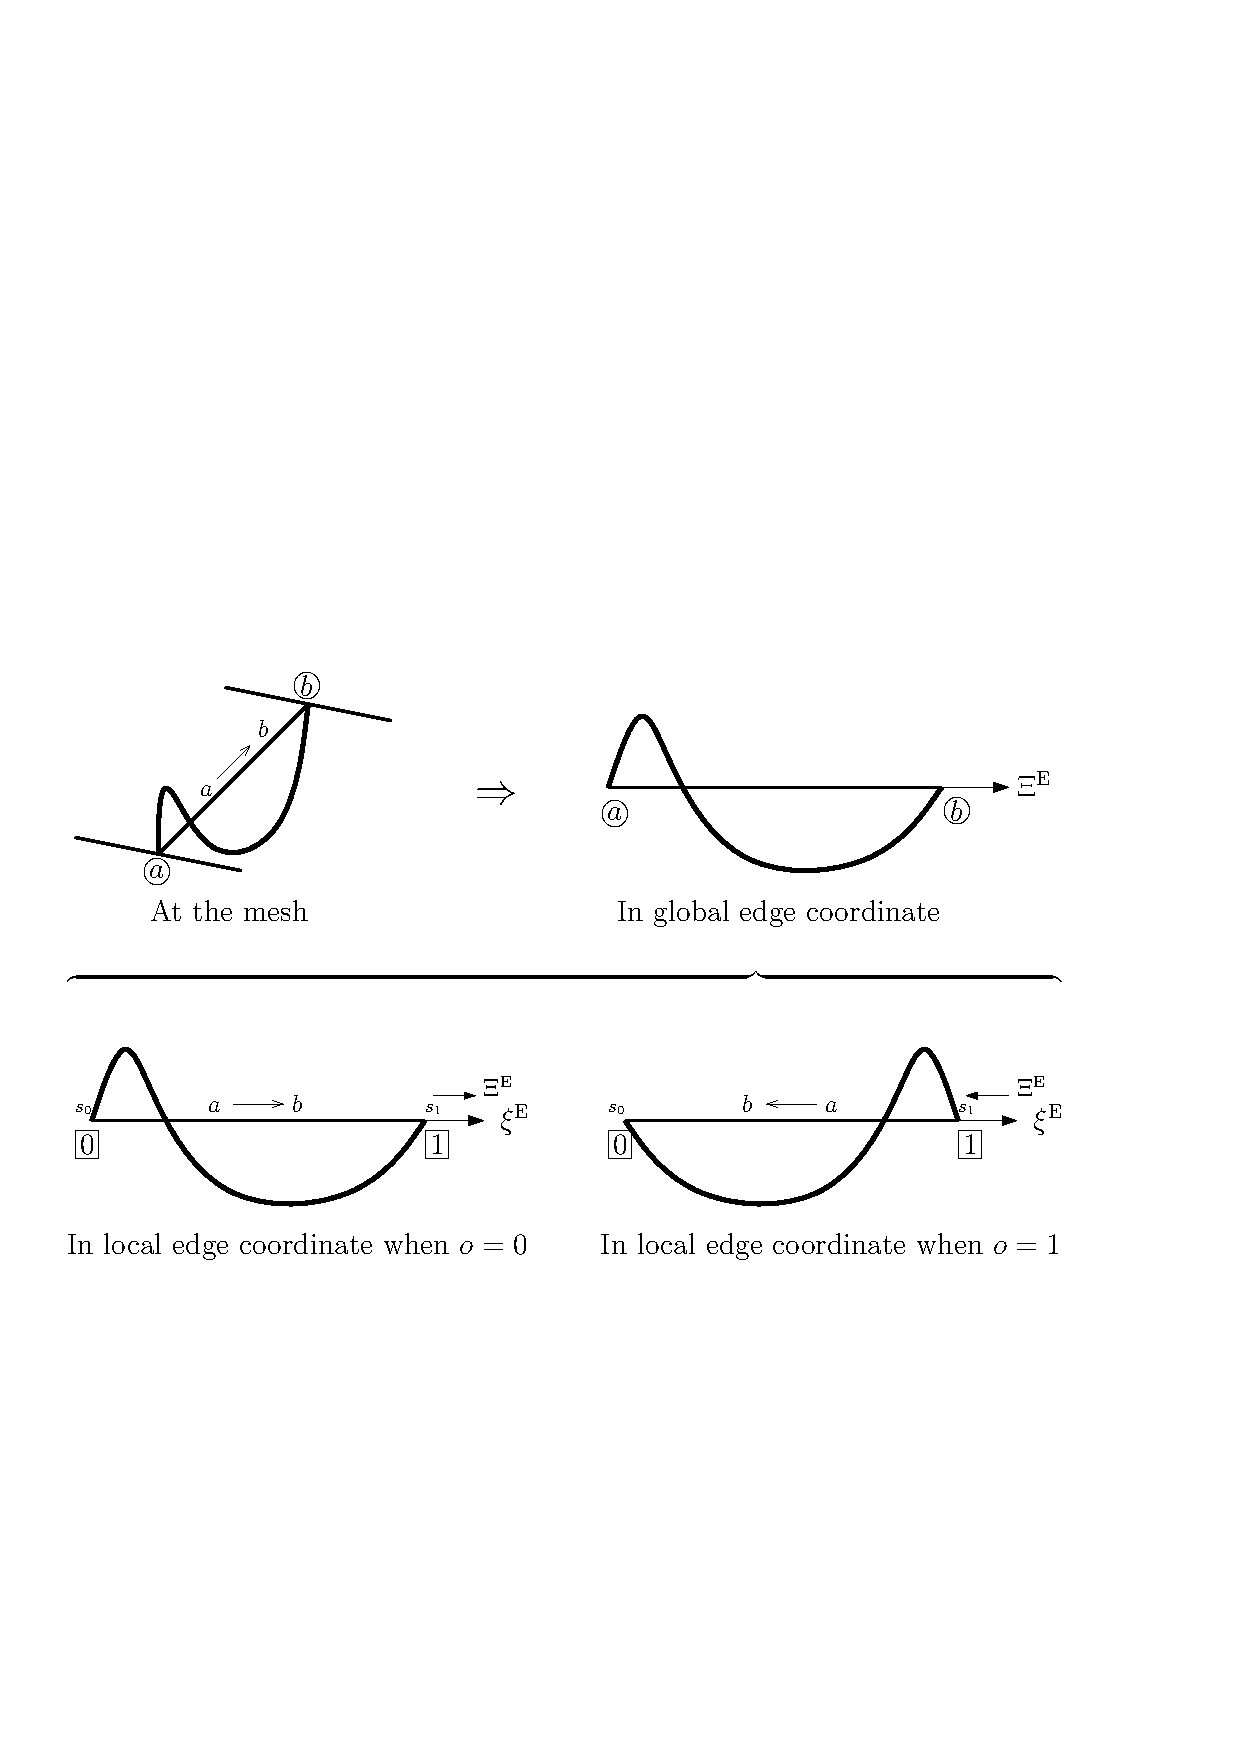
\includegraphics[scale=0.75]{./figures/OrientationsEdge.pdf}
\caption{Edge orientations.}
\label{fig:orientationsedge}
\end{center}
\end{figure}

%However, as the number of spatial dimensions increase, the trace will involve edge and face values over the elements.
%These \textit{do} have a concept of orientation.
%This makes the process of ``matching'' the trace of adjacent shape functions considerably more difficult.
In 2D, if one naively disregards how the elements are placed in the global mesh, and proceeds to define all shape functions at the (local) master element level, one might end up with shape functions that, when transformed back into the original mesh, are incompatible across shared edges (see Figure \ref{fig:edgemismatchintro}).
With orientation embedded shape functions this problem is avoided by taking into account more information of the global mesh. %when defining shape functions at the (local) master element.
This is done by giving each mesh edge its own \textit{global orientation}, and is represented by a global coordinate $\Xi^\E$, or equivalently by a \textit{global edge vertex-ordering}.
For example, given an edge at the mesh with vertices $a$ and $b$, a global edge vertex-ordering of the form $a\tto b$ means that $\Xi^\E$ has its origin at $a$ and points from $a$ to $b$.
This information is then passed to the particular master element, where the edge has its own fixed \textit{local orientation}, represented by the local coordinate $\xi^\E$, or equivalently by the the fixed \textit{local} edge vertex-ordering of the form $\boxednum{0}\!\tdashto\boxednum{1}$ (note the dashed arrow for \textit{local} orderings).
Viewed at the local level, the global coordinate $\Xi^\E$ can either coincide with the local coordinate $\xi^\E$ or point in the opposite direction.
To reflect these \textit{two} possibilities, the orientation parameter $\oo$ is introduced.
If $\oo=0$, this means the local and global coordinates coincide, and otherwise $\oo=1$.
%Notice that the global coordinate $\Xi^{\mathrm{e}}$ can be represented by the ordering of the vertices of the edge in the global mesh. This is referred to as the \textit{edge vertex-ordering}.
All this is depicted in Figure \ref{fig:orientationsedge}. % where the global orientation of the edge with vertices $a$ and $b$ is represented by the edge vertex-ordering $a\to b$, meaning that $\Xi^{\mathrm{e}}$ has its origin at $a$ and points from $a$ to $b$.
%This is shown in Figure \ref{fig:edgemismatch}.

%\begin{figure}[!ht]
%\begin{center}
%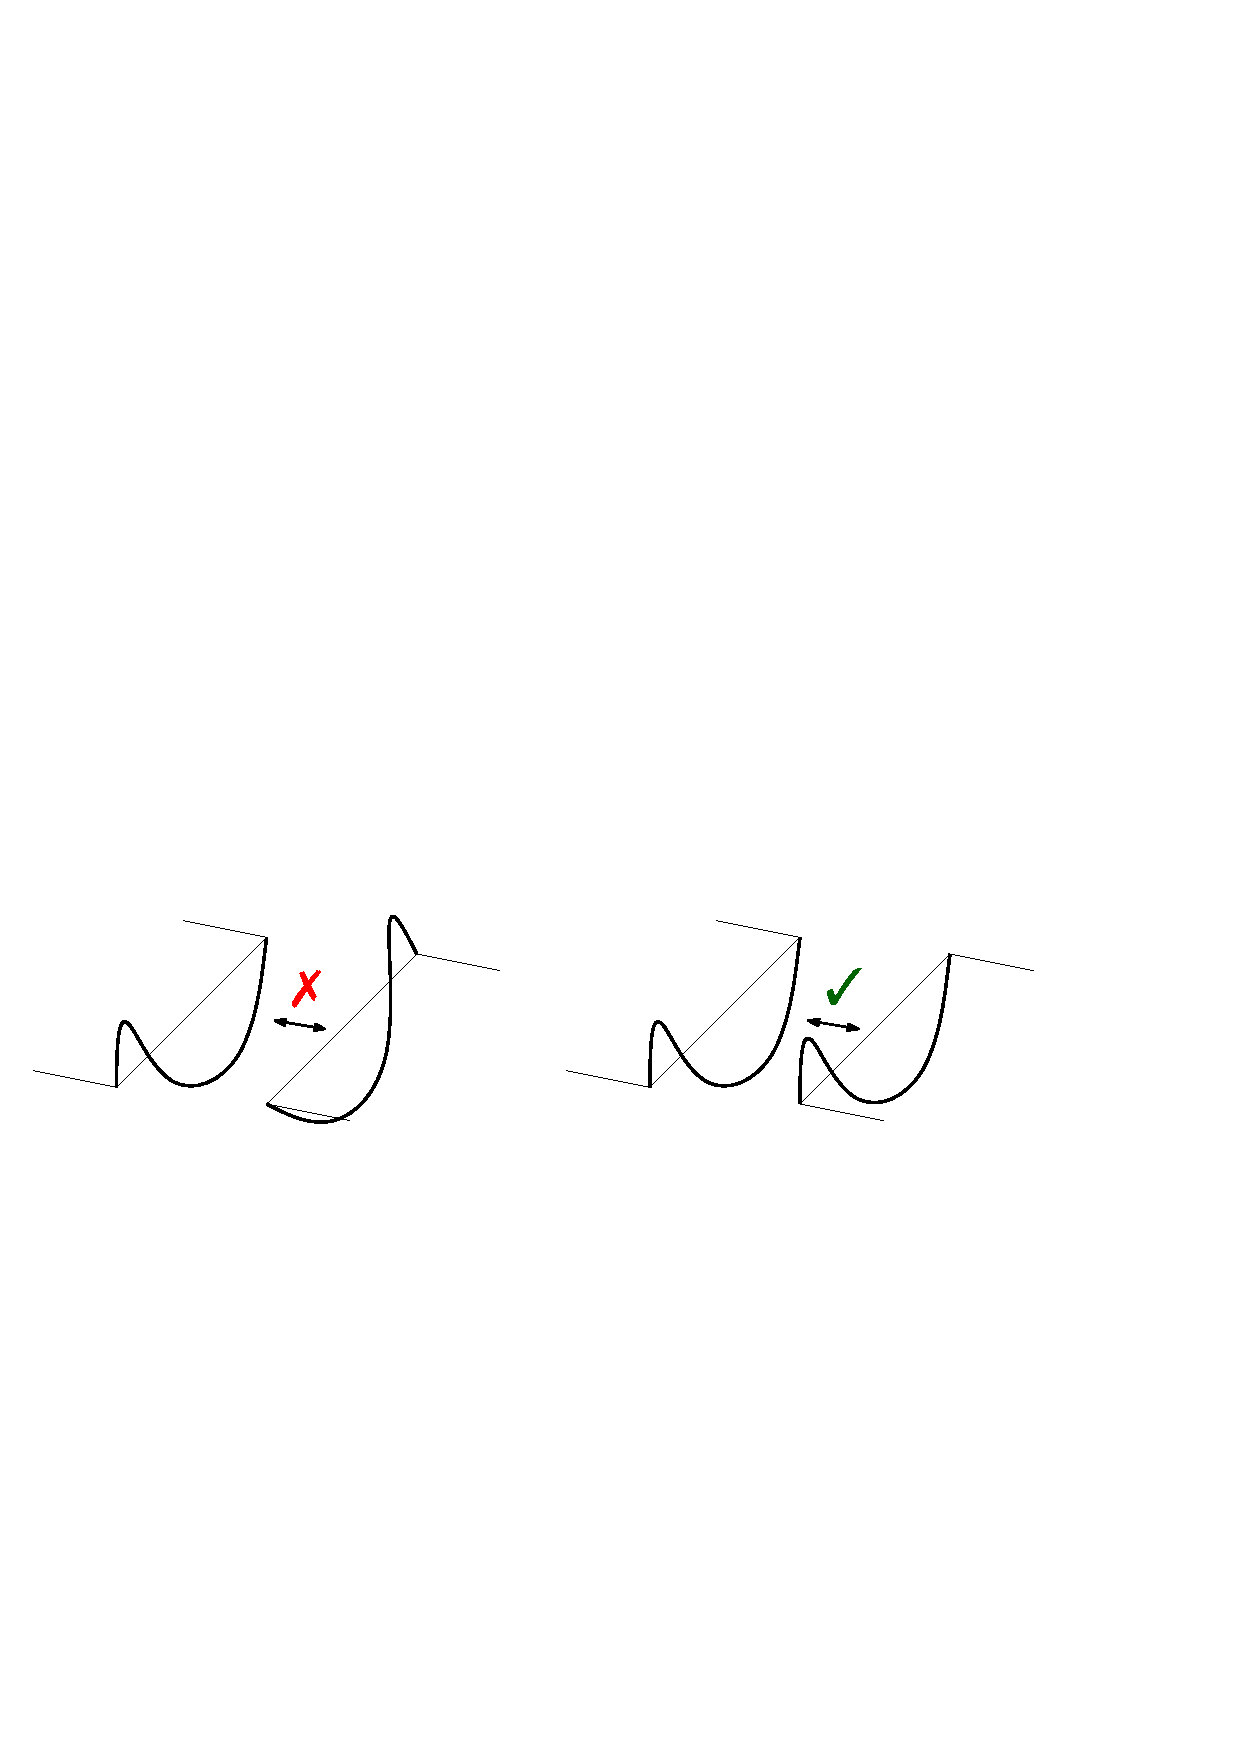
\includegraphics[scale=0.7]{./figures/OrientationsEdgeMismatch.pdf}
%\caption{Potential edge function mismatch in 2D due to disregarding the global mesh.}
%\label{fig:edgemismatch}
%\end{center}
%\end{figure}

%There are different ways to handle this issue.
%Traditionally it is done at the finite element assembly level.
%However, another practical alternative in many cases is to handle the problem at a much earlier point.
%This approach is called \textit{orientation embedding}.
%It consists of fixing or embedding an ``orientation'' to each relevant topological entity when the mesh is initially specified.

%For example, given a mesh in two dimensions, each edge is given its own ``orientation'', which corresponds to fixing a \textit{global edge axis} to each edge. It will be denoted by .
%In addition to this axis, there is a \textit{predefined local edge axis} for each edge at the master element level, denoted by $\xi^\mathrm{e}$.
%The edge shape function will have a fixed form when viewed from the global edge axis.
%Unfortunately, the shape function needs to be expressed in local axis coordinates, because these are associated to the master element and in turn to the integration procedure.
%Clearly the global edge axis only has two possibilities: it is either aligned with the local edge axis or it is not aligned.
%This is expressed by the orientation parameter $\oo$.
%If $\oo=0$ then the two axes are aligned, and if $\oo=1$ the two axes are not aligned. See Fig. (\textit{figure on orientation})

%The \textit{orientation embedded} shape functions are then constructed taking the extra orientation parameter $\oo$ into account.
%Note that shape functions are expressed in terms of master element coordinates, so the global orientation affects not only the function itself, but the derivative as well.

Due to the use of affine coordinates and the form of the ancillary functions proposed in this work, these orientation problems can be readily tackled.
To ensure full compatibility, we want the shape functions over a given edge to be immovable when observed in the global coordinates (like in Figure \ref{fig:orientationsedge}).
This is achieved by evaluating the ancillary functions with global coordinates.
Unfortunately, the available coordinates produced by the master element are the (fixed) local coordinates.
Hence, the idea is to apply a \textit{local-to-global transformation} over the edge, which will obviously depend on the orientation parameter $\oo$. 
Such a transformation is completely natural in the context of affine coordinates, since this only involves permutations of these coordinates.
Indeed, a simple permutation function dependent on $\oo$, denoted by $\sigma_\oo^\E$, will represent this transformation.

\begin{definition*}
Let $s_0$ and $s_1$ be arbitrary variables, and let $\oo=0,1$ be the edge orientation parameter. 
The edge orientation permutation function, $\sigma_\oo^\E$, is defined as
\begin{equation}
	\sigma_\oo^\E(s_0,s_1)=\begin{cases}\sigma_0^\E(s_0,s_1)=(s_0,s_1)&\quad\text{if  }\,\oo=0\,,\\
		\sigma_1^\E(s_0,s_1)=(s_1,s_0)&\quad\text{if  }\,\oo=1\,.\end{cases}\label{eq:orientEdge}
\end{equation}
\end{definition*}

%As expected, when $\oo=0$, there should be no changes, and this is reflected by $\sigma_\oo^\E$.
To explain the definition of $\sigma_\oo^\E$, note that in \eqref{eq:orientEdge}, if one links $s_0$ to the local vertex $\boxednum{0}$ and $s_1$ to the local vertex $\boxednum{1}$, then the \textit{locally ordered} pair $(s_0,s_1)$ represents the local coordinates.
It is ordered in the sense that $s_0$ comes first and $s_1$ comes second, and this is meant to correspond with the fixed \textit{local} ordering $\boxednum{0}\!\tdashto\boxednum{1}$, where $\boxednum{0}$ comes first and $\boxednum{1}$ comes second.
%It is ordered in the sense that just like in the fixed local ordering $\boxednum{0}\!\to\!\boxednum{1}\,$, first comes $\boxednum{0}$ and second comes $\boxednum{1}$, for the affine coordinates (the variables) first comes $s_0$ and second comes $s_1$.
Similarly, there are \textit{globally ordered} pairs which depend on the parameter $\oo$.
Indeed, in Figure \ref{fig:orientationsedge}, looking at the \textit{global} edge vertex-ordering $a\tto b$, there is an induced \textit{global} vertex-ordering of the two vertices $\boxednum{0}$ and $\boxednum{1}$.
It is $\boxednum{0}\!\tto\boxednum{1}$ if $\oo=0$, and $\boxednum{1}\!\tto\boxednum{0}$ if $\oo=1$.
Hence, the global coordinates are represented by the globally ordered pairs $(s_0,s_1)$ if $\oo=0$ and $(s_1,s_0)$ if $\oo=1$.
Therefore, in this sense, $\sigma_\oo^\E$ is a local-to-global transformation.

Now, all that is required is to compose the \textit{edge} ancillary functions and their differential form (those with superscript $\e$) with this permutation function $\sigma_\oo^\E$.
Thus, in 2D and 3D, all instances of $\phi_i^\E$ and $\nabla\phi_i^\E$ in the shape functions should be replaced with $\phi_i^\E\circ\sigma_\oo^\E$ and $\nabla\phi_i^\E\circ\sigma_\oo^\E$ respectively.
The resulting functions are then said to be \textit{orientation embedded} shape functions.
More concrete examples will be given in the 2D and 3D elements as the document progresses.


% the orientation $\oo$. Denoted by $\phi_i^{\e,\oo}$, the orientated ancillary function will be defined by permutations of the entries of the original function $\phi^\E_i$.
%Naturally, when $\oo=0$, the arguments of $\phi^\E_i$ are not permuted, while if $\oo=1$, the arguments are permuted.
%More explicitly,
%\begin{equation}
%    \phi_i^{\e,\oo}(s_0,s_1)=\begin{cases}\phi_i^{\e,0}(s_0,s_1)=\phi_i^{\e}(s_0,s_1)&\quad\text{if  }\,\oo=0\\
%        \phi_i^{\e,1}(s_0,s_1)=\phi_i^{\e}(s_1,s_0)&\quad\text{if  }\,\oo=1\,,\end{cases}\label{eq:edgeorientations}
%\end{equation}
%where $i=2,\ldots,p_s$. The same orientation rule applies for the derivatives and more generally to any function defined from now on which has a superscript $\e$.

%\begin{figure}[ht!]
%\centering
%%\includegraphics[width=\textwidth]{./figures/orientation.png}
%\caption{Two natural orientations of $E$.}
%\label{fig:EdgeOrientations}
%\end{figure}

%Given the functions $\mu_n$, $n=0,1$, defined in Equation~\eqref{eq:H1_1DAffine}, note that
%\[
%\mu_0+\mu_1 = 1\,, \quad \text{and}\quad \mu_n \geq 0\,,\, n=0,1
%\]
%at every point in $\e$. Therefore, $\mu_n$ are affine coordinates for $\e$.
%
%% We now concern ourselves with writing our edge functions, $\phi^\mathrm{e}_i$ as functions of affine coordinates.
%With an eye towards the coming  constructions, we define the orientation $\oo=0$ affine $H^1$ edge shape function as the homogenization of the Lobatto polynomials,
%\be
%\phi^\E_i(s_0,s_1) := \left[L_i\right] (s_0,s_1)\, , \quad i=2,\ldots,p\,.
%\label{eq:EdgeShap1}
%\ee
%Here, $s_0,\,s_0$, are arbitrary variables.
%Recalling the constraint $\mu_0+\mu_1=1$, we can reduce the equation above to,
%\be
%\phi^\E_i(\mu_0,\mu_1) = \left[L_i\right] (\mu_0,\mu_1) = L_i(\mu_1;\mu_0+\mu_1) = L_i(\mu_1),
%\ee
%when its arguments are affine functions of $\e$.
%
%Observe that orientation changes of the affine $H^1$ edge shape functions can be accounted for simply by permuting the ordering of the arguments in Equation~\eqref{eq:EdgeShap1} (see Figure~\ref{fig:EdgeOrientations})
%\be
%\phi^{\e,\oo}_i(\mu_0,\mu_1) =
%\left\{
%    \begin{array}{ll}
%        \left[L_i\right](\mu_0,\mu_1) = L_i(\mu_1) & \text{if } \oo = 0\\
%        \left[L_i\right](\mu_1,\mu_0) = L_i(\mu_0) & \text{if } \oo = 1
%    \end{array}
%\right.\,.
%\label{eq:1DOrientedAffineEdge}
%\ee
%
%Finally, we redefine the $1$D edge bubbles (with orientation accounted for) as
%\be
%\phi^\mathrm{e}_i(\xi) = \phi^{\e,\oo}_i(\mu_0(\xi),\mu_1(\xi))\,.
%\ee
%
%\paragraph*{Generalizations.}
%Here, we revisit Equation~\eqref{eq:EdgeShap1} to produce two general formulas which will arise in many shape functions constructions throughout the rest of the text.
%
%% \begin{remark}
%% We will see later the function $\phi^\E_i$ arise in many shape functions constructions. In other contexts,
%We will often find
%it necessary to consider the spatial gradient of $\phi^\E_i(s_0,s_1)$ where $s_n$, $n=0,1$, are functions of some spatial variable, $\xi$. We present the following general formula for future reference
%\begin{align}
%\bfnab_\xi \phi^\E_i\left(s_0,s_1\right) &= \bfnab_\xi L_i\left(s_1;s_0+s_1\right)
%\nonumber\\
%&= \frac{\ptl L_i}{\ptl x}\left(s_1;s_0+s_1\right) \bfnab_\xi s_1 + \frac{\ptl L_i}{\ptl t}\left(s_1;s_0+s_1\right) \bfnab_\xi\left(s_0+s_1\right)
%\nonumber\\
%% &= P_i\left(s_1(\xi);s_0(\xi)+s_1(\xi)\right) \bfnab_\xi s_1(\xi) + \frac{\ptl L_i}{\ptl t}\left(s_1(\xi);s_0(\xi)+s_1(\xi)\right) \bfnab_\xi\left(s_0(\xi)+s_1(\xi)\right)
%% \\
%&= \left[P_{i-1}\right]\left(s_0,s_1\right) \bfnab_\xi s_1 + \left[R_{i-1}\right]\left(s_0,s_1\right) \bfnab_\xi\left(s_0+s_1\right)\,.
%\label{eq:AffineEdgeGradient}
%\end{align}
%
%Moreover, we define the general, oriented, affine edge shape functions
%\be
%\phi^{\e,\oo}_i(s_0,s_1) =
%\left\{
%    \begin{array}{ll}
%        \left[L_i\right](s_0,s_1) & \text{if } \oo = 0\\
%        \left[L_i\right](s_1,s_0) & \text{if } \oo = 1
%    \end{array}
%\right.\,.
%\label{eq:OrientedAffineEdge}
%\ee
%Agreement of Equation~\eqref{eq:OrientedAffineEdge} with Equation~\eqref{eq:1DOrientedAffineEdge} is immediate.
%


% \end{remark}

% \begin{remark}
% Note that function $\phi_i$ in Equation~\eqref{eq:EdgeShap1} is not unique, but since each $\left[\phi_i\right]$ belong to the same equivalence class, the construction of the edge shape function, as a function of $\xi$ will be independent of the choice of $\phi_i$.
% \end{remark}
